% !TEX TS-program = pdflatex
% !TeX program = pdflatex
% !TEX encoding = UTF-8
% !TEX spellcheck = en_US

\documentclass[xcolor=table]{beamer}


%\usepackage{fullpage}
%\usepackage[left=2.8cm,right=2.2cm,top=2 cm,bottom=2 cm]{geometry}
\setbeamersize{text margin left=10pt,text margin right=10pt}



%\usepackage[T1]{fontenc}
\usepackage{textcomp}
\usepackage[utf8]{inputenc}
%\usepackage[french,english]{babel}
\usepackage{arabtex}
\usepackage{txfonts}
\usepackage{tipa}
\usepackage[]{graphicx}
\usepackage{multirow}
\usepackage{hyperref}
\usepackage{colortbl}
\usepackage{tabularray}
\usepackage{listingsutf8}
\usepackage{wrapfig}
\usepackage{multicol}
\usepackage[export]{adjustbox} %for images in table, also for frame
\usepackage[many]{tcolorbox}
\usepackage{wasysym}
\usepackage[lined]{algorithm2e}
\usepackage{alltt} %verbatim with commands
\usepackage{longtable}
\usepackage{tabu}

\usepackage{CJKutf8}

\usepackage{amsmath,amssymb, amsfonts} 

%\usepackage{newtxtext,newtxmath}


%\usepackage{acolor}


\definecolor{lightblue}{HTML}{D0D2FF}
\definecolor{lightyellow}{HTML}{FFFFAA}
\definecolor{darkblue}{HTML}{0000BB}
\definecolor{olivegreen}{HTML}{006600}
\definecolor{darkgreen}{HTML}{008B45} %009B55
\definecolor{violet}{HTML}{6600CC}
\definecolor{deeppink}{HTML}{FF1493}
\definecolor{orangey}{HTML}{FFBB00}


\makeatletter
\def\beamer@calltheme#1#2#3{%
	\def\beamer@themelist{#2}
	\@for\beamer@themename:=\beamer@themelist\do
	{\IfFileExists{\beamer@themelocation/#3\beamer@themename.sty}{%
	\usepackage[{#1}]{\beamer@themelocation/#3\beamer@themename}}{\usepackage[{#1}]{#3\beamer@themename}}
		
	}%
}

\def\usefolder#1{
	\def\beamer@themelocation{#1}
}
\def\beamer@themelocation{}
\makeatother

\usefolder{../../extra/beamer-themes}

\usetheme{Karim} % Antibes Boadilla Warsaw Karim

\beamertemplatenavigationsymbolsempty

\let\oldcite\cite
\renewcommand{\cite}[1]{{\bfseries\color{blue}\oldcite{#1}}}

\tcbuselibrary{listings}


%\renewcommand{\baselinestretch}{1.5}

\def\supit#1{\raisebox{0.8ex}{\small\it #1}\hspace{0.05em}}

\AtBeginSection{%
	\begin{frame}
		\sectionpage
	\end{frame}
}

\newcommand{\rottext}[2]{%
	\rotatebox{90}{%
	\begin{minipage}{#1}%
		\raggedleft#2%
	\end{minipage}%
	}%
}


\institute{ %
Laboratoire de la Communication dans les Systèmes Informatiques (LCSI)
\par
École  nationale Supérieure d'Informatique (ESI), Algiers, Algeria
}
\author[Abdelkrime Aries (2023/2024)] %
{Abdelkrime Aries}
%\titlegraphic{
\includegraphics[height=1cm]{../img/esi-logo.png}%\hspace*{4.75cm}~


\date{Academic year: 2023/2024} %\today

\titlegraphic{%
	
\includegraphics[height=1cm]{../../img/misc/esi-logo.png}%
	\hspace{2cm}%
	
\includegraphics[height=1cm]{../../img/misc/lcsi-logo.png}%
	\hspace{2cm}%
	
\includegraphics[height=1.5cm]{../../img/misc/esi.nlp-logo.png}%
}

%\setbeamertemplate{headline}{}

\newcommand{\kurl}[1]{{\scriptsize\bfseries\color{orangey}\url{#1}}}

\newcommand{\keyword}[1]{\textcolor{red}{\bfseries\itshape #1}}
\newcommand{\expword}[1]{\textcolor{olivegreen}{#1}}
\newcommand{\optword}[1]{\textcolor{violet}{\bfseries #1}}

\makeatletter
\newcommand\mysphere{%
	\parbox[t]{10pt}{\raisebox{0.2pt}{\beamer@usesphere{item projected}{bigsphere}}}}
\makeatother

%\let\oldtabular\tabular
%\let\endoldtabular\endtabular
%\renewenvironment{tabular}{\rowcolors{2}{white}{lightblue}\oldtabular\rowcolor{blue}}{\endoldtabular}


%\NoAutoSpacing %french autospacing after ":"

\def\graphpath{}

\newcommand{\changegraphpath}[1]{\def\graphpath{#1}}


\newcommand{\vgraphpage}[2][.84\textheight]{%
%	\begin{center}%
		\includegraphics[height=#1]{\graphpath #2}%
%	\end{center}%
}

\newcommand{\hgraphpage}[2][\textwidth]{%
%	\begin{center}%
		\includegraphics[width=#1]{\graphpath #2}%
%	\end{center}%
}

\newcommand{\graphpage}[2][]{%
	\includegraphics[#1]{\graphpath #2}%
}

\bibliographystyle{apalike}

\newcommand{\insertbibliography}[2]{
	\appendix
	\section*{Bibliography}
	\nocite{#2}
%	\makeatletter % to change template
%	\setbeamertemplate{headline}[default] % not mandatory, but I though it was better to set it blank
%	\def\beamer@entrycode{\vspace*{-\headheight}} % here is the part we are interested in :)
%	\makeatother
	\begin{multicols*}{2}[\frametitle{\insertsection} \usebeamertemplate*{frametitle}]%\usebeamertemplate*{frametitle}\frametitle{Références}
		\tiny
		\bibliography{#1}
	\end{multicols*}
}

\definecolor{my-grey}{RGB}{233, 233, 233}

\newcommand{\insertlicence}{
	\begin{frame}[plain]
	\frametitle{License: CC-BY 4.0}

	\begin{tcolorbox}[colback=cyan,
		colframe=cyan,  
		arc=0pt,outer arc=0pt,
		valign=top, 
		halign=center,
		width=\textwidth]
		
		
\includegraphics[width=.5cm]{../../img/licence/cc_icon_white_x2.png}
		
\includegraphics[width=.5cm]{../../img/licence/attribution_icon_white_x2.png}
		
		\color{white}
		\bfseries Attribution 4.0 International (CC BY 4.0) \\
		\tiny \url{https://creativecommons.org/licenses/by/4.0/deed.en}
		
	\end{tcolorbox}\vspace{-.5cm}
	\begin{tcolorbox}[colback=my-grey,
		colframe=my-grey,  
		center, arc=0pt,outer arc=0pt,
		valign=top, 
		halign=left,
		width=\textwidth]
		
		\tiny
		
		\begin{center}
			\bfseries\Large
			You are free to:
		\end{center}
		
		\begin{minipage}{0.83\textwidth}
			\begin{itemize}
				\item[] \textbf{Share} — copy and redistribute the material in any medium or format
				\item[] \textbf{Adapt} — remix, transform, and build upon the material
				for any purpose, even commercially.
			\end{itemize}
		
			\vspace{12pt}
		
			\textit{The licensor cannot revoke these freedoms as long as you follow the license terms.}
		\end{minipage}
		\begin{minipage}{0.15\textwidth}
			
\includegraphics[width=\textwidth]{../../img/licence/FreeCulturalWorks_seal_x2.jpg}
		\end{minipage}
	
		
		\begin{center}
			\bfseries\Large
			Under the following terms:
		\end{center}
		
		\begin{itemize}
			\item[] \textbf{Attribution} — You must give appropriate credit, provide a link to the license, and indicate if changes were made. You may do so in any reasonable manner, but not in any way that suggests the licensor endorses you or your use.
			\item[] \textbf{No additional restrictions} — You may not apply legal terms or technological measures that legally restrict others from doing anything the license permits.
		\end{itemize}
		
	\end{tcolorbox}
	
%	\begin{center}
%		\bfseries Attribution 4.0 International (CC BY 4.0)
%		\url{https://creativecommons.org/licenses/by/4.0/deed.fr}
%	\end{center}

%	\tiny
%
%	Vous êtes autorisé à : 
%	\begin{itemize}
%		\item \textbf{Partager} — copier, distribuer et communiquer le matériel par tous moyens et sous tous formats
%		\item \textbf{Adapter} — remixer, transformer et créer à partir du matériel
%	\end{itemize}
%	
%	Selon les conditions suivantes : 
%	\begin{itemize}
%		\item \textbf{Attribution} — Vous devez créditer l'Œuvre, intégrer un lien vers la licence et indiquer si des modifications ont été effectuées à l'Oeuvre. Vous devez indiquer ces informations par tous les moyens raisonnables, sans toutefois suggérer que l'Offrant vous soutient ou soutient la façon dont vous avez utilisé son Oeuvre.
%		\item \textbf{Pas d'Utilisation Commerciale} — Vous n'êtes pas autorisé à faire un usage commercial de cette Oeuvre, tout ou partie du matériel la composant. 
%		\item \textbf{Pas de restrictions complémentaires} — Vous n'êtes pas autorisé à appliquer des conditions légales ou des mesures techniques qui restreindraient légalement autrui à utiliser l'Oeuvre dans les conditions décrites par la licence.
%	\end{itemize}

	\end{frame}
}

\settowidth{\leftmargini}{\usebeamertemplate{itemize item}}
\addtolength{\leftmargini}{\labelsep}

\AtBeginDocument{
	\newcolumntype{L}[2]{>{\vbox to #2\bgroup\vfill\flushleft}p{#1}<{\egroup}} 
	
	\begin{frame}[plain]
		\maketitle
	\end{frame}

	\insertlicence
}


% needs etoolbox; to break links after -
\appto\UrlBreaks{\do\-}


\makeatletter
\newcommand{\xRightarrow}[2][]{\ext@arrow 0359\Rightarrowfill@{#1}{#2}}
\makeatother


\usefonttheme{structurebold}
%\usefonttheme{professionalfonts}


% figure caption
\setlength\abovecaptionskip{2pt}

% equations
\AtBeginDocument{
\abovedisplayskip=0pt
\abovedisplayshortskip=0pt
\belowdisplayskip=0pt
\belowdisplayshortskip=0pt
}


\title[ESI - NLP(master): 02- ML for NLP]%
{Natural Language Processing (Master)\\Chapter 02\\Machine learning for NLP} 

\changegraphpath{../../img/ml4nlp/}

\begin{document}
	
%	\begin{frame}
%		\frametitle{Traitement automatique du langage naturel}
%		\framesubtitle{ML for NLP : Introduction}
%		
%		
%	\end{frame}
	
	\begin{frame}
		\frametitle{Natural Language Processing}
		\framesubtitle{ML for NLP: Algorithms and abbreviations}
		
		\begin{itemize}
			\item \optword{NB}: Naive Bayes
			\item \optword{LR}: Logistic regression
			\item \optword{SVM}: Support-Vector Machine
			\item \optword{NN}: Neural Network
			\item \optword{FFN}: Feed Forward Network
			\begin{itemize}
				\item \optword{MLP}: Multi-Layer Perceptron
				\item \optword{CNN}: Convolutional Neural Network
			\end{itemize}
			\item \optword{RNN}: Recurrent Neural Network
			\item \optword{HMM}: Hidden Markov Model
			\item \optword{MEMM}: Maximum-Entropy Markov Model
			\item \optword{CRF}: Conditional Random Field
		\end{itemize}
		
	\end{frame}
	
	\begin{frame}
		\frametitle{Natural Language Processing}
		\framesubtitle{ML for NLP: Types of models}
		
		\scriptsize
		\begin{tblr}{
				colspec = {p{.12\textwidth}lp{.37\textwidth}lp{.38\textwidth}},
				row{odd} = {lightblue},
				row{1} = {darkblue, fg=white, font=\bfseries, valign=m, halign=c},
				column{2,4}={white},
				column{1}={bg=darkblue, fg=white, font=\bfseries, valign=m},
				row{even} = {white},
				cell{1}{1}={white},
				colsep=3pt,
				rowsep=3pt,
				stretch = 0,
			}
			
			&& Generative && Discriminative \\
			
			&&&&\\
			
			Text && NB && LR, SVM, MLP, RNN, CNN \\
			
			&&&&\\
			
			Sequence && HMM  && MEMM, CRF, RNN \\
			
		\end{tblr}
		
		\vfill
		
		\begin{itemize}
			\item \optword{Generative model}: a model that learns to generate features given a class:
			\[\hat{Y} = \arg\max_k P(Y_k) P(X | Y_k)\]
			
			\item \optword{Discriminative model}: a model that learns to estimate a class given some features: 
			\[\hat{Y} = \arg\max_k P(Y_k | X)\]
		\end{itemize}
		
	\end{frame}
	
	
	\begin{frame}
		\frametitle{Natural Language Processing}
		\framesubtitle{ML for NLP: Plan}
		
		\begin{multicols}{2}
			%	\small
			\tableofcontents
		\end{multicols}
	\end{frame}
	
	%===================================================================================
	\section{Machine learning}
	%===================================================================================
	
	\begin{frame}
		\frametitle{ML for NLP}
		\framesubtitle{\insertsection}
		
		\begin{itemize}
			\item This section is a review of ML algorithms
			\item Traditional ML algorithms: LR, SVM, DT, NB
			\begin{itemize}
				\item Text features are engineered manually
			\end{itemize}
			\item MLP (Multi-Layer Perceptron)
			\begin{itemize}
				\item Text features can be learned/enhanced automatically
				\item The terminology is wrongly used to refer to Fully connected feed-forward neural networks with at least three layers
			\end{itemize}
			\item CNN (Convolutional Neural Network)
			\begin{itemize}
				\item Extracting relations between consecutive units
			\end{itemize}
			\item RNN (Recurrent Neural Network)
			\begin{itemize}
				\item Temporal dependent units processing
			\end{itemize}
		\end{itemize}
		
	\end{frame}

	\begin{frame}
		\frametitle{ML for NLP}
		\framesubtitle{\insertsection: Example (Simple Perceptron for binary logical functions)}
		
		\begin{minipage}{0.30\textwidth} 
			\hgraphpage{perceptron.pdf}
		\end{minipage}
		%
		\begin{minipage}{0.59\textwidth}
			\scriptsize
			\begin{itemize}
				\item $ z^{(i)} = x_1^{(i)} w_1 + x_2^{(i)} w_2 + b $
				\item $ \hat{y}^{(i)} = \phi(z^{(i)}) = \begin{cases}
					1 & \text{if } z^{(i)} \ge 0 \\
					0 & \text{otherwise}
				\end{cases} $
				\item $ w_j = w_j + \nabla w_j$ where $ \nabla w_j = \frac{1}{M}\sum_{i=0}^{M} (y^{(i)} - \hat{y}^{(i)}) * x_j^{(i)} $
			\end{itemize}
		\end{minipage}
	
		\vfill
	
		\begin{exampleblock}{Training a Perceptron for AND function}
			\begin{minipage}{0.2\textwidth} 
				\scriptsize
				\begin{tabular}{|c|c|c|}
					\hline
					x\textsubscript{1} & x\textsubscript{2} & y \\
					\hline
					0 & 0 & 0  \\
					\hline
					0 & 1 & 0 \\
					\hline
					1 & 0 & 0 \\
					\hline
					1 & 1 & 1 \\
					\hline
				\end{tabular}
			\end{minipage}
			%
			\begin{minipage}{0.79\textwidth}
				\scriptsize
				\begin{itemize}
					\item Initially, $ W = [w_1, w_2, b] = [0, 0, 0] $.
					
					\item It1: $ Z = \hat{Y} = [0, 0, 0, 0] $, 
					$ \nabla W = [\frac{1}{4}, \frac{1}{4}, \frac{1}{4}] $, 
					$ W = [\frac{1}{4}, \frac{1}{4}, \frac{1}{4}] $.
					
					\item It2: $ Z = [\frac{1}{4}, \frac{2}{4}, \frac{2}{4}, \frac{3}{4}] $, 
					$ \hat{Y} = [1, 1, 1, 1] $, 
					$ \nabla W = [\frac{-1}{4}, \frac{-1}{4}, \frac{-3}{4}] $,
					$ W = [0, 0, \frac{-1}{2}] $.
					
					\item It3: $ Z = [\frac{-1}{2}, \frac{-1}{2}, \frac{-1}{2}, \frac{-1}{2}] $, 
					$ \hat{Y} = [1, 1, 1, 1] $, 
					$ \nabla W = [\frac{1}{4}, \frac{1}{4}, \frac{1}{4}] $,
					$ W = [\frac{1}{4}, \frac{1}{4}, \frac{-1}{4}] $.
					
					\item It4: $ Z = [\frac{-1}{4}, 0, 0, \frac{1}{4}] $, 
					$ \hat{Y} = Y = [0, 0, 0, 1] $ (STOP)
				\end{itemize}
			\end{minipage}
		\end{exampleblock}
		
	\end{frame}
	
	\subsection{Traditional ML}
	
	\begin{frame}
		\frametitle{ML for NLP: \insertsection}
		\framesubtitle{\insertsubsection}
	
		\begin{itemize}
%			\item Features are engineered manually 
			\item The classification model stores some parameters $\theta$
			\begin{itemize}
				\item They are used by an inference function $ f $ to find the perfect class.
				\item They can be considered to be some rules on the input to find the output.
				\item Eg. \expword{IF weather = warm THEN play}
			\end{itemize}
			\item These parameters are trained using an algorithm based on some data
			\begin{itemize}
				\item They are tuned so the model find the exact output of the data
			\end{itemize}
			\item The data is a table of samples, features and class
			\begin{itemize}
				\item Let's consider $ M $ samples (rows) and $ N $ features (columns)
				\item $ X[M, N] $ is the input
				\item $ Y[M] $ is the output
			\end{itemize}
			\item In summary, to infer a class $ \hat{y} $ of a sample $ x $
			\[\hat{y} = f(x, \theta)\]
		\end{itemize}
		
	\end{frame}

	\begin{frame}
		\frametitle{ML for NLP: \insertsection}
		\framesubtitle{\insertsubsection: Linear Regression}
		
		\begin{minipage}{0.62\textwidth} 
			\begin{itemize}
				\item \textbf{GOAL}: Try to estimate a value $ y $ based on some features $ x $
				\item \textbf{Estimation}: $ \hat{y} = \theta_0 + \sum_{j=1}^{N} \theta_j x_j $
				\item \textbf{Training}: Try to minimize a cost function $ J $
				\[J_\theta = \frac{1}{2M} \sum\limits_{i=1}^{M} (y^{(i)} - \hat{y}^{(i)})^2\]
%				\item $J_\theta = \frac{1}{M} \sum\limits_{i=1}^{M} (y^{(i)} - \hat{y}^{(i)})^2$
%				\item Eg. \expword{Houses prices based on their areas}
			\end{itemize}
		\end{minipage}
		\begin{minipage}{0.37\textwidth} 
			\hgraphpage{houses_LR.png}
		\end{minipage}
		
		\begin{itemize}
			
			\item Update each parameter $ \theta_j $ iteratively using a learning rate $ \alpha $
			\[\theta_j = \theta_j - \alpha \frac{\partial J_\theta}{\partial \theta_j}
			\hspace{1cm}
			\frac{\partial J_\theta}{\partial \theta_j} = \frac{1}{M} \sum\limits_{i=1}^{M} (\hat{y}^{(i)} - y^{(i)}) x_j
			\]
			\item The update is stopped when the cost is minimal
		\end{itemize}
	
	\end{frame}

	\begin{frame}
		\frametitle{ML for NLP: \insertsection}
		\framesubtitle{\insertsubsection: Linear Regression (Cost and parameters)}
		
		\begin{minipage}{0.7\textwidth} 
			\begin{block}{Gradient descent}
				\begin{algorithm}[H]
					\KwData{$ X, Y, \alpha, T $}
					\KwResult{$ \theta $}
					initialize $ \theta $ ; $ t = 0 $\;
					calculate $ J $\;
					\While{$ t < T$ and $ J \ge tol $}{
						$ \theta = \theta - \alpha \Delta_\theta J(X, Y; \theta) $\;
						calculate $ J $\;
						t = t + 1 \;
					}
%					\caption{Gradient descent}
				\end{algorithm}
			\end{block}
		\end{minipage}
		\begin{minipage}{0.29\textwidth} 
			\hgraphpage{J.pdf}
		\end{minipage}
		
		%		\begin{itemize}
			%			\item \textbf{Training}: Try to minimize a cost function $ J $
			%			\[J_\theta = \frac{-1}{M} \sum\limits_{i=1}^{M} y^{(i)} \log(h^{(i)}) + (1- y^{(i)}) \log(1 - h^{(i)})\]
			%			\item Update each parameter $ \theta_j $ iteratively using a learning rate $ \alpha $
			%			\[\theta_j = \theta_j - \alpha \frac{\partial J_\theta}{\partial \theta_j}
			%			\hspace{1cm}
			%			\frac{\partial J_\theta}{\partial \theta_j} = \frac{1}{M} \sum\limits_{i=1}^{M} (\hat{y}^{(i)} - y^{(i)}) x_j
			%			\]
			%			%			\item The update is stopped when the cost is minimal
			%		\end{itemize}
		
	\end{frame}

	\begin{frame}
		\frametitle{ML for NLP: \insertsection}
		\framesubtitle{\insertsubsection: Binary Logistic Regression}
		
		\begin{minipage}{0.5\textwidth} 
			\hgraphpage{LR_bin_arch.pdf}
		\end{minipage}
		\begin{minipage}{0.49\textwidth} 
			\hgraphpage{exp_binary.pdf}
		\end{minipage}
		
	\end{frame}

	\begin{frame}
		\frametitle{ML for NLP: \insertsection}
		\framesubtitle{\insertsubsection: Binary Logistic Regression (Formalism)}
		
		\begin{minipage}{0.5\textwidth} 
			\begin{itemize}
				\item \textbf{GOAL}: Try to draw a decision line between two classes $ y \in \{0, 1\} $ based on some features $ x $
				\item \textbf{Estimation}: $ z = \theta_0 + \sum_{j=1}^{N} \theta_j x_j $
				$ h = \sigma(z) = \frac{1}{1 + e^{-z}}$, $ \hat{y} = (h \ge 0.5)$
			\end{itemize}
		\end{minipage}
		\begin{minipage}{0.49\textwidth} 
			\hgraphpage{grades_LR.png}
		\end{minipage}
		
		\begin{itemize}
			\item \textbf{Training}: Try to minimize a cost function $ J $
			\[J_\theta = \frac{-1}{M} \sum\limits_{i=1}^{M} y^{(i)} \log(h^{(i)}) + (1- y^{(i)}) \log(1 - h^{(i)})\]
			\item Update each parameter $ \theta_j $ iteratively using a learning rate $ \alpha $
			\[\theta_j = \theta_j - \alpha \frac{\partial J_\theta}{\partial \theta_j}
			\hspace{1cm}
			\frac{\partial J_\theta}{\partial \theta_j} = \frac{1}{M} \sum\limits_{i=1}^{M} (\hat{y}^{(i)} - y^{(i)}) x_j
			\]
%			\item The update is stopped when the cost is minimal
		\end{itemize}
		
	\end{frame}

	\begin{frame}
		\frametitle{ML for NLP: \insertsection}
		\framesubtitle{\insertsubsection: Multinomial Logistic Regression}
		
		\begin{minipage}{0.6\textwidth} 
			\hgraphpage{LR_multi_arch.pdf}
		\end{minipage}
		\begin{minipage}{0.39\textwidth} 
			\hgraphpage{exp_multiclass.pdf}
		\end{minipage}
		
	\end{frame}
	
	\begin{frame}
		\frametitle{ML for NLP: \insertsection}
		\framesubtitle{\insertsubsection: Multinomial Logistic Regression (Formalism)}
		
		\begin{minipage}{0.7\textwidth} 
			\begin{itemize}
				\item \textbf{GOAL}: Try to draw decision lines between many classes $ y $ based on some features $ x $
				\item \textbf{Estimation}: $ z_l = \theta_{0l} + \sum_{j=1}^{N} \theta_{jl} x_j $
				$ h_l = Softmax(z_l) = \frac{e^{z_l}}{\sum_{k=1}^{L} e^{z_k}}$, $ \hat{y} = \arg\max_{l} h_l$
				\item \textbf{Also}: $ L $ binary logistic classifiers. 
				The probabilities are normalized: $ \sum_{l=1}^{L} p(c_l) = 1$.
%				Each estimates a probability of a class $ c_l $.
%				Then, these probabilities are normalized to have normalized probabilities $ \sum_{l=1}^{L} p(c_l) = 1$.
			\end{itemize}
		\end{minipage}
		\begin{minipage}{0.29\textwidth} 
			\hgraphpage{multi_LR.pdf}
		\end{minipage}
	
		\begin{itemize}
			\item \textbf{Training}: Try to minimize a cost function $ J $
			\[J_\theta = \frac{-1}{M} \sum\limits_{i=1}^{M} \sum_{k=1}^{L} h^{(i)}_k \log(h^{(i)}_k)
			\hspace{1cm}
			\frac{\partial J_\theta}{\partial \theta_{jl}} = \frac{1}{M} \sum\limits_{i=1}^{M} (h_l^{(i)} - y_l^{(i)}) x_j
			\]
		\end{itemize}
		
	\end{frame}

	\begin{frame}
		\frametitle{ML for NLP: \insertsection}
		\framesubtitle{\insertsubsection: Support-Vector Machine (Primal form)}
		
		\begin{minipage}{0.75\textwidth} 
			\begin{itemize}
				\item \textbf{GOAL}: Try to draw a decision line between two classes $ y $ based on some features $ x $ like LR. But, in this case the margin between the two classes must be maximal.
				\item \textbf{Estimation}: $ z = b + \sum_{j=1}^{N} \theta_j x_j $, 
				$ \hat{y} = (z \ge 0.5)$
			\end{itemize}
		\end{minipage}
		\begin{minipage}{0.24\textwidth} 
			\hgraphpage{SVM_primal.pdf}
		\end{minipage}
		
		\begin{itemize}
			\item \textbf{Training}: Try to minimize a cost function $ J $, $ y \in \{-1, 1\} $
			\[J_\theta = \frac{1}{M} \left[ \frac{1}{2}||\theta||^2 + C \sum\limits_{i=1}^{M} \max (0, 1 - y^{(i)} z^{(i)}) \right]
%			\hspace{1cm}
%			\frac{\partial J_\theta}{\partial \theta_{jl}} = \frac{1}{M} \sum\limits_{i=1}^{M} (h_l^{(i)} - y_l^{(i)}) x_j
			\]
			
			\[\frac{\partial J_\theta}{\partial \theta_{j}} = \frac{1}{M} \left[ \theta_j + \sum\limits_{i=1}^{M} \begin{cases}
				0 & \text{if } y^{(i)} z^{(i)} \ge 1\\
				- C x^{(i)}_j y^{(i)} & \text{otherwise}  \\
			\end{cases} \right]
			\]
		\end{itemize}
		
	\end{frame}
	
	\begin{frame}
		\frametitle{ML for NLP: \insertsection}
		\framesubtitle{\insertsubsection: Support-Vector Machine (Dual form)}
		
		\begin{minipage}{0.75\textwidth} 
			\begin{itemize}
				\item \textbf{GOAL}: The same as Primal form's, but a new sample is represented by its similarity to training samples
				\item \textbf{Estimation}: 
				\[\hat{y_t} = sign(\sum^M_{i=1} \alpha_i y^{(i)} K(x^{(i)}, x_t) - b)\]
			\end{itemize}
		\end{minipage}
		\begin{minipage}{0.24\textwidth} 
			\hgraphpage{SVM_dual.pdf}
		\end{minipage}
	
	
		\begin{itemize}
			\item \textbf{Training}: Try to minimize a cost function $ J $
			\[J_\alpha = \sum\limits_{i=1}^{M} \alpha_i - \frac{1}{2} \sum\limits_{i=1}^{M} \sum\limits_{j=1}^{M} \alpha_i \alpha_j y^{(i)} y^{(j)} K(x^{(i)}, x^{(j)})\]
			\item $\alpha$ and $ b $ are updated using an optimization algorithm like \keyword{Sequential minimal optimization}
		\end{itemize}
		
	\end{frame}

	\begin{frame}
		\frametitle{ML for NLP: \insertsection}
		\framesubtitle{\insertsubsection: Decision Trees}
		
		\vspace{-8pt}
		\begin{exampleblock}{Example of expected model}
		\begin{minipage}{0.33\textwidth} 
			\tiny\bfseries
			\SetTblrInner{rowsep=0pt,colsep=1pt}
			\begin{tblr}{
					colspec = {llllll},
					row{odd} = {lightblue},
					row{even} = {lightyellow},
					row{1} = {bg=darkblue, fg=white},
				} 
%			\begin{tabular}{llllll}
				id & outlook & temp & humidity & windy & play \\
				01 & sunny & hot & high & false & no \\
				02 & sunny & hot & high & true & no \\
				03 & overcast & hot & high & false & yes \\
				04 & rainy & mild & high & false & yes \\
				05 & rainy & cool & normal & false & yes \\
				06 & rainy & cool & normal & true & no \\
				07 & overcast & cool & normal & true & yes \\
				08 & sunny & mild & high & false & no \\
				09 & sunny & cool & normal & false & yes \\
				10 & rainy & mild & normal & false & yes \\
				11 & sunny & mild & normal & true & yes \\
				12 & overcast & mild & high & true & yes \\
				13 & overcast & hot & normal & false & yes \\
				14 & rainy & mild & high & true & no \\
%			\end{tabular}
			\end{tblr}
		\end{minipage}
		\begin{minipage}{0.25\textwidth} 
			\tiny\bfseries\itshape
			\textcolor{red}{if} outlook == '\textcolor{darkgreen}{sunny}':\\
			\hspace*{10pt}\textcolor{red}{if}  humidity == '\textcolor{darkgreen}{high}':\\
			\hspace*{20pt}\textcolor{red}{return}  '\textcolor{darkgreen}{no}'\\
			\hspace*{10pt}\textcolor{red}{else}: \textcolor{gray}{\# 'normal'}\\
			\hspace*{20pt}\textcolor{red}{return} '\textcolor{darkgreen}{yes}'\\
			\textcolor{red}{elif}  outlook == '\textcolor{darkgreen}{overcast}':\\
			\hspace*{10pt}\textcolor{red}{return} '\textcolor{darkgreen}{yes}'\\
			\textcolor{red}{else}: \textcolor{gray}{\# 'rainy'}\\
			\hspace*{10pt}\textcolor{red}{if not} windy:\\
			\hspace*{20pt}\textcolor{red}{return} '\textcolor{darkgreen}{yes}'\\
			\hspace*{10pt}\textcolor{red}{else}:\\
			\hspace*{20pt}\textcolor{red}{return} '\textcolor{darkgreen}{no}' 
		\end{minipage}
		\begin{minipage}{0.38\textwidth} 
			 \hgraphpage{exp_DT.pdf}
		\end{minipage}
		\end{exampleblock}
		
		\vspace{-6pt}
		\begin{itemize}
			\item \textbf{GOAL}: Create a tree by splitting the training data. The leafs must contain homogeneous samples (same class)
			\item \textbf{Estimation}: navigate the tree from the root till a leaf based on the sample's features
		\end{itemize}
		
	\end{frame}

	\begin{frame}
		\frametitle{ML for NLP: \insertsection}
		\framesubtitle{\insertsubsection: Decision Trees (Training)}
	
		\begin{block}{Decision tree construction}
			\scriptsize
			\begin{algorithm}[H]
				\SetKwFunction{FConst}{build}
				\SetKwProg{Fn}{function}{}{end}
				
				\KwData{$ X, Y$}
				\KwResult{Decision tree's root node} 
				\Return \FConst{$X, Y$}\;
				
				\Fn{\FConst{$X', Y'$}}{
					n $\leftarrow$ new Node()\;
					\eIf{$Y'$ is homogeneous or stop criteria is reached}{
						$s.class \leftarrow \arg\max_{k}{|\{y \in Y' / y = k \}|}$ \tcp{$s$ is a leaf}
					}{
						determine the feature $j$ of $ X' $ which better divides $Y'$\;
						split $(X, Y)$ into $(X_1, Y_1), \ldots, (X_K, Y_K)$ based on the $ K $ values of $X'_j$\;
						$s.feature = j$\;
						\lForEach{$ k \in \{1, \ldots, K\}$}{
%							$s_k \leftarrow Construction(X_{*,k}, Y_k) \in S$ $(s, s_k) \in A$ $val(s, s_k) = k$\;
							$ n.children[k] \leftarrow$ \FConst{$ X_k, Y_k $})
						}
					}
					
					\Return n\;
				}	
				
%				\caption{Génération d'un arbre de décision (algorithme général)}
			\end{algorithm}
		\end{block}
		
	\end{frame}

	\begin{frame}
		\frametitle{ML for NLP: \insertsection}
		\framesubtitle{\insertsubsection: Decision Trees (ID3: Iterative Dichotomiser 3)}
		
		\begin{itemize}
			\item \textbf{LEARN MORE}: \cite{1986-quinlan}
			\item Probability of a given value $ v $ belonging into a set $ S $
			\[p(v\in S) = \frac{|\{x / x\in S \text{ and } x = v\}|}{|S|}\]
			\item Entropy: uncertainty of a set $ S $ having a set $ V $ of unique values
			\[H(S) = - \sum\limits_{v \in V} p(v\in S) \log_2 p(v\in S)\]
			\item Information gain: difference in entropy from before to after the set $ S $ is split on an attribute $ A $ with $ V $ unique values.
			\[IG(Y, A) = H(Y) - \sum_{v \in V} p(v\in A) H(Y_{v\in A})\] 
		\end{itemize}
	
		\[H(Y) = 0 \Rightarrow\ Y \text{ is homogeneous} \hspace{1cm} j_{best} = \arg\max_j IG(Y, X_j)\]
		
	\end{frame}

	\begin{frame}
		\frametitle{ML for NLP: \insertsection}
		\framesubtitle{\insertsubsection: Decision Trees (ID3 - Example and application)}
		\tiny
		\begin{enumerate}
			\item Create a node $ ROOT $
			\begin{itemize}\tiny\bfseries
				\item $ H(Y) = - p(yes \in Y) \log_2 p(yes\in Y) - p(no \in Y) \log_2 p(no\in Y)  $
				$ = -\frac{9}{14} \log_2 \frac{9}{14} - \frac{5}{14} \log_2 \frac{5}{14} \approx\ 0.94$ (not pure)
%				\item $ IG(Y, outlook) = H(Y) - \sum_{v \in \{sunny, overcast, rainy\}} p(v\in A) H(Y_{v\in outlook}) $
				\item $ IG(Y, outlook) = 0.94 - [ \underbrace{\frac{5}{14} (- \frac{3}{5} \log_2 \frac{3}{5} - \frac{2}{5} \log_2 \frac{2}{5} )}_{sunny} + \underbrace{\frac{4}{14} (- \frac{0}{4} \log_2 \frac{0}{4} - \frac{4}{4} \log_2 \frac{4}{4})}_{overcast} +  \underbrace{\frac{5}{14} (- \frac{2}{5} \log_2 \frac{2}{5} - \frac{3}{5} \log_2 \frac{3}{5})}_{rainy} ]$
				\item $ IG(Y, outlook) \approx 0.247 , IG(Y, temp) \approx 0.029 , IG(Y, humidity) \approx 0.152 ,  IG(Y, wind) \approx 0.048 $ (outlook is the best)
				\item split the dataset into three datasets ($ X_1, X_2, X_3 $), each will be used to create a child of $ ROOT $
			\end{itemize}
		
			\item Create a node $ N_1 $ where $ X_1, Y_1 $ are split on $ X[outlook] = sunny$ (5 samples)
			\begin{itemize}\tiny\bfseries
				\item $ H(Y_1) = - \frac{3}{5} \log_2 \frac{3}{5} - \frac{2}{5} \log_2 \frac{2}{5} \approx\ 0.97$ (not pure)
				\item $ IG(Y_1, temp) = 0.97 - [ \underbrace{\frac{2}{5} (- \frac{2}{2} \log_2 \frac{2}{2} - \frac{0}{2} \log_2 \frac{0}{2} )}_{hot} + \underbrace{\frac{2}{5} (- \frac{1}{2} \log_2 \frac{1}{2} - \frac{1}{2} \log_2 \frac{1}{2})}_{mild} +  \underbrace{\frac{1}{5} (- \frac{0}{1} \log_2 \frac{0}{1} - \frac{1}{1} \log_2 \frac{1}{1})}_{cool} ]$
				\item $ IG(Y_1, temp) \approx 0.57 , IG(Y_1, humidity) \approx 0.97 ,  IG(Y_1, wind) \approx 0.02 $ (humidity is the best)
				\item split the dataset into two datasets ($ X_{11}, X_{12}$), each will be used to create a child of $ N_1 $
			\end{itemize}
		
			\item Create a node $ N_2 $ where $ X_2, Y_2 $ are split on $ X[outlook] = overcast$ (4 samples)
			\begin{itemize}\tiny\bfseries
				\item $ H(Y_2) = - \frac{0}{4} \log_2 \frac{0}{4} - \frac{4}{4} \log_2 \frac{4}{4} = 0$ (pure: one class)
				\item $ N_2.class = 'yes' $
			\end{itemize}
		
		\end{enumerate}
	\end{frame}

	\begin{frame}
		\frametitle{ML for NLP: \insertsection}
		\framesubtitle{\insertsubsection: Naive Bayes}
		
		\begin{itemize}
			\item Bayes' theorem: $ \overbrace{p(y|x)}^\text{Posterior} = \frac{\overbrace{p(y)}^\text{Prior} \overbrace{p(x|y)}^{\text{Likelihood}}}{\underbrace{p(x)}_\text{Evidence}}$
			\item \textbf{GOAL}: Estimate classes' probabilities based on features' distributions
			\item \textbf{Estimation}: $ \hat{y} = \arg\max_{y_l} p(y_l|x)$
			\[\hat{y} = \arg\max_{y_l} \frac{p(y_l) p(x|y_l)}{\underbrace{p(x)}_\text{constant}} = \arg\max_{y_l} p(y_l) p(x|y_l)\]
			\begin{itemize}
				\item the \textbf{naive} part: we suppose features' independence
				\[\hat{y} = \arg\max_{y_l} p(y_l) \prod_{j=1}^{N} p(x_j|y_l) = \arg\max_{y_l} \log p(y_l) + \sum_{j=1}^{N} \log p(x_j|y_l)\]
			\end{itemize}
		\end{itemize}
		
	\end{frame}

	\begin{frame}
		\frametitle{ML for NLP: \insertsection}
		\framesubtitle{\insertsubsection: Naive Bayes (training) (1)}
		\small
		
		\begin{itemize}
			\item \optword{Prior probability}: let $ Y $ be the training outputs
			\[p(y_k) = \frac{|\{y / y \in Y \wedge y = k\}|}{|Y|}\]
			
			\item \optword{Likelihood probability (Multinomial NB)} let $ Y $ be the training outputs, let $ x_j $ be a feature, let $ v $ be an acceptable value of $ x_j $.
			\[p(x_j = v|y_k) = \frac{|\{y^{(i)} / y^{(i)} = k \wedge x^{(i)}_j = v\}|}{|\{y | y \in Y \wedge y = k\}|} = \frac{\#(y = k \wedge x_j = v)}{\#(y = k)}\]
			
			Some values $v$ may not be in training dataset. We can smooth the probability using the unique values $ V_j $ of $ x_j $ and $ \alpha \in [0, 1] $
			\[p(x_j = v|y_k) = \frac{\#(y = k \wedge x_j = v) + \alpha}{\#(y = k) + \alpha |V_j|}\]
		\end{itemize}
		
	\end{frame}

	\begin{frame}
		\frametitle{ML for NLP: \insertsection}
		\framesubtitle{\insertsubsection: Naive Bayes (training) (2)}
		\small
		
		\begin{itemize}
			\item \optword{Likelihood probability (Bernoulli NB)}: let $ Y $ be the training outputs, let $ x_j $ be a feature, let $ v \in \{0, 1\}$ be an acceptable value of $ x_j $.
			\[p(x_j = v|y_k) = p(x_{j1}|y_k) x_j + (1-p(x_{j1}|y_k)) (1-x_j)\]
			\[p(x_{j1}|y_k) = \frac{|\{x_j^{(i)} = 1 \wedge y^{(i)} = k\}|}{|\{y | y \in Y \wedge y = k\}|}\]
			\item \optword{Likelihood probability (Gaussian NB)}: let $ Y $ be the training outputs, let $ x_j $ be a feature, let $ v $ be an acceptable value of $ x_j $.
			\[p(x_j = v|y_k) = \frac{1}{\sqrt{2\pi \sigma_{kj}^2}} e^\frac{-(v-\mu_{kj})^2}{2 \sigma_{kj}^2}\]
		\end{itemize}
		
	\end{frame}

	\begin{frame}
		\frametitle{ML for NLP: \insertsection}
		\framesubtitle{\insertsubsection: Some humor}
		
		\begin{center}
			\vgraphpage{humor/humor-tradutional_ml.jpg}
		\end{center}
		
	\end{frame}
	
	\subsection{MLP}
	
	\begin{frame}
		\frametitle{ML for NLP: \insertsection}
		\framesubtitle{\insertsubsection}
		
		\begin{minipage}{0.39\textwidth}
			\centering 
			Artificial Neuron Architecture
			
			\hgraphpage{aneuron.pdf}
		\end{minipage}
		\begin{minipage}{0.4\textwidth} 
			\centering
			MLP architecture
			
			\hgraphpage{RN.pdf}
		\end{minipage}
		
		\begin{minipage}{0.39\textwidth}
			\[z_j^{(l)} = \sum_i w_{ij}^{(l)} a_{i}^{(l-1)} + b_{i}^{(l)}\]
			
			\[a_{i}^{(l)} = f_{i}^{(l)}(z_{i}^{(l)})\]
			
			\[a_{i}^{(1)} = x_{i}\]
		\end{minipage}
		\begin{minipage}{0.6\textwidth} 
			\centering
			MLP notation
			
			\hgraphpage{RNPA.pdf}
		\end{minipage}
		
	\end{frame}
	
	\begin{frame}
		\frametitle{ML for NLP: \insertsection}
		\framesubtitle{\insertsubsection: Feed-Forward}
		
		\begin{minipage}{0.3\textwidth}
			\small
			
			Simplify chain rule\boldmath
			
			$ \delta^{(out)} = \frac{\partial J}{\partial f^{(out)}} \frac{\partial f^{(out)}}{\partial z^{(out)}} $
			
			$ \delta^{(l)} = \frac{\partial f^{(l)}}{\partial z^{(l)}} w^{(l+1)} \delta^{(l+1)} $
			
			$ \frac{\partial J}{\partial w^{(l)}} = a^{(l-1)} \delta^{(l)} $
			
			$ \frac{\partial J}{\partial b^{(l)}} = \delta^{(l)} $
			
		\end{minipage}
		\begin{minipage}{0.69\textwidth} 
			\hgraphpage{RNPA-exp.pdf}
		\end{minipage}
		
		\begin{minipage}{0.45\textwidth} 
			\tiny
			$
			\frac{\partial J}{\partial w_{11}^{(4)}} = \overbrace{\frac{\partial J}{\partial f_{1}^{(4)}} \frac{\partial f_{1}^{(4)}}{\partial z_{1}^{(4)}}}^{\delta_{1}^{(4)}} \overbrace{\frac{\partial z_{1}^{(4)}}{\partial w_{11}^{(4)}}}^{a_{1}^{(3)}}
			$
			
			$ 
			\frac{\partial J}{\partial f_{1}^{(4)}} = \frac{(0.840, 0.843) - (0, 1)}{(0.840, 0.843) - (0.840, 0.843)^2} 
			= (6.25, -1.186)
			$
			
			$ 
			\frac{\partial f_{1}^{(4)}}{\partial z_{1}^{(4)}} = (0.840, 0.843) (0.160, 0.157) = (0.134, 0.132)
			$
			
			$
			\delta_{1}^{(4)} = (6.25, -1.186) (0.134, 0.132) \approx (0.838, -0.157)
			$ 
		\end{minipage}
		\begin{minipage}{0.54\textwidth} 
			\tiny
			$
			\frac{\partial J}{\partial w_{11}^{(3)}} = 
			\overbrace{
				\overbrace{
					\frac{\partial J}{\partial f_{1}^{(4)}} 
					\frac{\partial f_{1}^{(4)}}{\partial z_{1}^{(4)}}
				}^{\delta_{1}^{(4)}} 
				\overbrace{
					\frac{\partial z_{1}^{(4)}}{\partial f_{1}^{(3)}}
				}^{w_{11}^{(4)}} 
				\frac{\partial f_{1}^{(3)}}{\partial z_{1}^{(3)}} 
			}^{\delta_{1}^{(3)}} 
			\overbrace{
				\frac{\partial z_{1}^{(3)}}{\partial w_{11}^{(3)}}
			}^{a_{1}^{(2)}}
			$
			
			$
			\frac{\partial f_{1}^{(3)}}{\partial z_{1}^{(3)}} \approx 
			(0.555, 0.612) (0.445, 0.388) = (0.247, 0.237)
			$
			
			$
			\delta_{1}^{(3)} = (0.838, -0.157) * 0.7 * (0.247, 0.237) \approx (0.145, -0.026)
			$
		\end{minipage}
		
		
	\end{frame}

	\begin{frame}
		\frametitle{ML for NLP: \insertsection}
		\framesubtitle{\insertsubsection: Auto-encoder}
		
		\begin{minipage}{0.47\textwidth}
			\hgraphpage{AE.pdf}
		\end{minipage}
		\hfill
		\begin{minipage}{0.47\textwidth} 
			\hgraphpage{AE-noise.pdf}
		\end{minipage}
		
		\begin{minipage}{0.52\textwidth}
			\small
			$ z = \mu + \sigma * N(0, 1) $
			
			\vspace{6pt}$ J'(x, \hat{x}) = J(x, \hat{x}) + KL(N(\mu, \sigma), N(0, 1)) $
			
			\vspace{6pt}$ KL(p||q) = \sum_i p(x_i) log(\frac{p(x_i)}{q(x_i)}) $
		\end{minipage}
		\begin{minipage}{0.47\textwidth} 
			\hgraphpage{AE-var.pdf}
		\end{minipage}
		
		
	\end{frame}

	\begin{frame}
		\frametitle{ML for NLP: \insertsection}
		\framesubtitle{\insertsubsection: Some humor}
		
		\begin{center}
			\vgraphpage{humor/humor-nn.jpg}
		\end{center}
		
	\end{frame}
	
	
	\subsection{CNN}
	
	\begin{frame}
		\frametitle{ML for NLP: \insertsection}
		\framesubtitle{\insertsubsection: Traditional image processing}
		
		\begin{center}
			\hgraphpage[\textwidth]{img-learn.pdf}
		\end{center}
		
	\end{frame}
	
	\begin{frame}
		\frametitle{ML for NLP: \insertsection}
		\framesubtitle{\insertsubsection: Convolution (principle)}
		
		\begin{itemize}
			\item An image is a matrix of pixels.
			\item Convolution: modify the value of a pixel with respect to its neighbors.
			\item two parameters: \optword{padding} (surround the image with 0s to preserve its original size), \optword{stride} (the kernel/mask shifting step).
		\end{itemize}
		
		\begin{center}
			\hgraphpage[.8\textwidth]{conv.pdf}
		\end{center}
		
	\end{frame}
	
	\begin{frame}
		\frametitle{ML for NLP: \insertsection}
		\framesubtitle{\insertsubsection: Conv2D}
		
		\begin{minipage}{0.60\textwidth} 
			\begin{itemize}
				\item Image's spatial structure is maintained.
				\item The layer learns one or more kernels.
				\item $ w' = \frac{w - w_f + 2P}{S} + 1$,  $ h' = \frac{h - h_f + 2P}{S} + 1$.
				\item Filters number $k$ can be specified.
				\item Parameters number will be $w_f * h_f * c * k$ plus $k$ bias.
				\item E.g., \expword{image: 32x32x3; kernel: 5x5; s: 1; p: 0; k: 6.}. In this case, we will have \expword{456} parameters to train.
			\end{itemize}
		\end{minipage}
		%
		\begin{minipage}{0.39\textwidth}
			\hgraphpage[\textwidth]{conv2d.pdf}
		\end{minipage}
		
	\end{frame}

	\begin{frame}
		\frametitle{ML for NLP: \insertsection}
		\framesubtitle{\insertsubsection: Conv2D (Example)}
		
		\begin{center}
			\vskip-6pt\hgraphpage[0.8\textwidth]{conv2D_imlp.pdf}
		\end{center}\vskip-16pt
		
		{\scriptsize 
			\[O_{11} = ReLU(\Sigma = b + F_{11} I_{11} + \textcolor{blue}{F_{12} I_{12}} + F_{21} I_{21} + \textcolor{red}{F_{22} I_{22}})  \]
			\[O_{12} = ReLU(\Sigma = b + \textcolor{blue}{F_{11} I_{12}} + F_{12} I_{13} + \textcolor{red}{F_{21} I_{22}} + F_{22} I_{23})  \]
			\[O_{21} = ReLU(\Sigma = b + F_{11} I_{21} + \textcolor{red}{F_{12} I_{22}} + F_{21} I_{31} + F_{22} I_{32})  \]
			\[O_{22} = ReLU(\Sigma = b + \textcolor{red}{F_{11} I_{22}} + F_{12} I_{23} + F_{21} I_{32} + F_{22} I_{33})  \]
			
			\[\textcolor{red}{\frac{\partial J}{\partial I_{22}}} 
			= \underbrace{\frac{\partial J}{\partial O_{11}}}_{G_{11} = 1} 
			\underbrace{\frac{\partial ReLU}{\partial \sum}}_{1} 
			\underbrace{\frac{\partial \sum}{\partial I_{22}}}_{F_{22} = 3}
			+ \underbrace{\frac{\partial J}{\partial O_{12}}}_{G_{12} = 2} 
			\underbrace{\frac{\partial ReLU}{\partial \sum}}_{1} 
			\underbrace{\frac{\partial \sum}{\partial I_{22}}}_{F_{21} = -2}
			+ \underbrace{\frac{\partial J}{\partial O_{21}}}_{G_{21} = 3} 
			\underbrace{\frac{\partial ReLU}{\partial \sum}}_{1} 
			\underbrace{\frac{\partial \sum}{\partial I_{22}}}_{F_{12} = -1}
			+ \underbrace{\frac{\partial J}{\partial O_{22}}}_{G_{22} = 4} 
			\underbrace{\frac{\partial ReLU}{\partial \sum}}_{0} 
			\underbrace{\frac{\partial \sum}{\partial I_{22}}}_{F_{11} = 1}\]
			
			\[\textcolor{blue}{\frac{\partial J}{\partial I_{12}}} 
			= \underbrace{\frac{\partial J}{\partial O_{11}}}_{G_{11} = 1} 
			\underbrace{\frac{\partial ReLU}{\partial \sum}}_{1} 
			\underbrace{\frac{\partial \sum}{\partial I_{12}}}_{F_{12} = -1}
			+ \underbrace{\frac{\partial J}{\partial O_{12}}}_{G_{12} = 2} 
			\underbrace{\frac{\partial ReLU}{\partial \sum}}_{1} 
			\underbrace{\frac{\partial \sum}{\partial I_{12}}}_{F_{11} = 1}\]
		}
		
	\end{frame}

	\begin{frame}
		\frametitle{ML for NLP: \insertsection}
		\framesubtitle{\insertsubsection: Conv1D}
		
		\begin{minipage}{0.62\textwidth} 
			\begin{itemize}
				\item Like \keyword{Conv2D}, but it generates a vector
				\item Kernel's width is equal to original width
				\item $ h' = \frac{h - h_f + 2P}{S} + 1$. $ w' = 1$.
				\item Filters number $k$ can be specified.
				\item Parameters number will be $w * h_f * k$ plus $k$ bias.
				\item E.g., \expword{text: 32x3; kernel: 5; s: 1; p: 0; k: 6.}. In this case, we will have \expword{96} parameters to train.
			\end{itemize}
		\end{minipage}
		%
		\begin{minipage}{0.37\textwidth}
			\hgraphpage[\textwidth]{conv1d.pdf}
		\end{minipage}
		
	\end{frame}
	
	\begin{frame}
		\frametitle{ML for NLP: \insertsection}
		\framesubtitle{\insertsubsection: Pooling}
		
		\begin{minipage}{0.60\textwidth} 
			\begin{itemize}
				\item Make the representation smaller and more manageable.
				\item $ w' = \frac{w - w_f + 2P}{S} + 1$,  $ h' = \frac{h - h_f + 2P}{S} + 1$
				\item No parameters 
				\item \optword{Max Pool}: the gradient is passed only to the winning cell (which has the max).
				\item \optword{Average Pool}: the gradient is equally passed to he participating cells: $\frac{\text{gradient}}{w_f * h_f}$ 
			\end{itemize}
		\end{minipage}
		%
		\begin{minipage}{0.39\textwidth}
			\hgraphpage[\textwidth]{maxpool.pdf}
		\end{minipage}
		
	\end{frame}

	\begin{frame}
		\frametitle{ML for NLP: \insertsection}
		\framesubtitle{\insertsubsection: Pooling (Example)}
		
		\begin{center}
			\vskip-6pt\hgraphpage[0.7\textwidth]{pool2D_imlp.pdf}
		\end{center}\vskip-16pt
		
		{\scriptsize 
			\[O_{11} = Max(I_{11} + \textcolor{blue}{I_{12}} + I_{21} + \textcolor{red}{I_{22}}) = \textcolor{red}{I_{22}}  \]
			\[O_{12} = Max(\textcolor{blue}{I_{12}} + I_{13} + \textcolor{red}{I_{22}} + I_{23}) = I_{23}  \]
			\[O_{21} = Max(I_{21} + \textcolor{red}{I_{22}} + I_{31} + I_{32}) = \textcolor{red}{I_{22}} \]
			\[O_{22} = Max(\textcolor{red}{I_{22}} + I_{23} + I_{32} + I_{33}) = \textcolor{red}{I_{22}}  \]
			
			\[\textcolor{red}{\frac{\partial J}{\partial I_{22}}} 
			= \underbrace{\frac{\partial J}{\partial O_{11}}}_{G_{11} = 1} 
			\underbrace{\frac{\partial Max}{\partial I_{22}}}_{1}
			+ \underbrace{\frac{\partial J}{\partial O_{12}}}_{G_{12} = 2} 
			\underbrace{\frac{\partial Max}{\partial I_{22}}}_{0}
			+ \underbrace{\frac{\partial J}{\partial O_{21}}}_{G_{21} = 3} 
			\underbrace{\frac{\partial Max}{\partial I_{22}}}_{1}
			+ \underbrace{\frac{\partial J}{\partial O_{22}}}_{G_{22} = 4} 
			\underbrace{\frac{\partial Max}{\partial I_{22}}}_{1}\]
			
			\[\textcolor{blue}{\frac{\partial J}{\partial I_{12}}} 
			= \underbrace{\frac{\partial J}{\partial O_{11}}}_{G_{11} = 1} 
			\underbrace{\frac{\partial Max}{\partial I_{12}}}_{0}
			+ \underbrace{\frac{\partial J}{\partial O_{12}}}_{G_{12} = 2} 
			\underbrace{\frac{\partial Max}{\partial I_{12}}}_{0}\]
		}
		
	\end{frame}

	\begin{frame}
		\frametitle{ML for NLP: \insertsection}
		\framesubtitle{\insertsubsection: Some humor}
		
%		\begin{center}
			\hgraphpage{humor/humor-conv2d.png}
%		\end{center}
		
	\end{frame}
	
	\subsection{RNN}
	
	\begin{frame}
		\frametitle{ML for NLP: \insertsection}
		\framesubtitle{\insertsubsection: Architecture}
		
		\begin{minipage}{0.49\textwidth} 
			\begin{itemize}
				\item \optword{Elman network}
				\begin{align*}
					h_t = f(w_x x_t + w_h \textcolor{red}{h_{t-1}} + b_h) \\
					\hat{y}_t = g(w_y h_t + b_y)
				\end{align*}
				\item \optword{Jordan network}
				\begin{align*}
					h_t = f(w_x x_t + w_h \textcolor{red}{\hat{y}_{t-1}} + b_h) \\
					\hat{y}_t = g(w_y h_t + b_y)
				\end{align*}
			\end{itemize}
		\end{minipage}
		%
		\begin{minipage}{0.5\textwidth}
			\hgraphpage[\textwidth]{RNN.pdf}
		\end{minipage}
		
	\end{frame}
	
	\begin{frame}
		\frametitle{ML for NLP: \insertsection}
		\framesubtitle{\insertsubsection: Applications}
		
		\begin{tabular}{p{.32\textwidth}p{.15\textwidth}p{.4\textwidth}}
%			\hline\hline
			\textbf{Type} & \textbf{Illustration} & \textbf{Example} \\
%			\hline
			Many to many & 
			\vgraphpage[1.4cm, valign=c]{RNNpp1.pdf} & 
			Named entity detection \\
			
%			\hline
			Many to many (Seq2seq) & 
			\vgraphpage[1.4cm, valign=c]{RNNpp2.pdf} & 
			Machine translation \\
			
%			\hline
			Many to one & 
			\vgraphpage[1.4cm, valign=c]{RNNp1.pdf} & 
			Sentiment classification \\
			
%			\hline
			One to many & 
			\vgraphpage[1.4cm, valign=c]{RNN1p.pdf} & 
			Image caption generation \\
			
%			\hline\hline
			
		\end{tabular}
		
	\end{frame}

	\begin{frame}
		\frametitle{ML for NLP: \insertsection}
		\framesubtitle{\insertsubsection: Back-propagation example (many2many)}
		
		\[ h_t = f(x_t, h_{t-1}, W_x, W_h),\,\,\, \hat{y}_t = g(h_t, W_y),\,\,\,  J(\hat{y}, y) = \frac{1}{T} \sum_{t=1}^{T} j(\hat{y}_t, y_t)\]
		
		\begin{minipage}{0.6\textwidth}\scriptsize
			\begin{align*}
				\frac{\partial J}{\partial W_h} & = \frac{1}{T} \sum_{t=1}^{T} \frac{\partial j(\hat{y}_t, y_t)}{\partial W_h}
				= \frac{1}{T} \sum_{t=1}^{T} \frac{\partial j(\hat{y}_t, y_t)}{\partial \hat{y}_t} 
				\frac{\partial g(h_t, W_y)}{\partial h_t} 
				\frac{\partial h_t}{\partial W_h} \\
				\frac{\partial h_t}{\partial W_h} & = 
				\frac{\partial f(x_t, h_{t-1}, W_x, W_h)}{\partial W_h} + 
				\frac{\partial f(x_t, h_{t-1}, W_x, W_h)}{\partial h_{t-1}} \frac{\partial h_{t-1}}{\partial W_h} \\
				\frac{\partial J}{\partial W_y} & =
				\frac{1}{T} \sum_{t=1}^{T} \frac{\partial j(\hat{y}_t, y_t)}{\partial W_y}
				= \frac{1}{T} \sum_{t=1}^{T} \frac{\partial j(\hat{y}_t, y_t)}{\partial \hat{y}_t} 
				\frac{\partial g(h_t, W_y)}{\partial W_y} \\
				\frac{\partial J}{\partial W_x} & = 
				\frac{1}{T} \sum_{t=1}^{T} \frac{\partial j(\hat{y}_t, y_t)}{\partial W_x}
				= \frac{1}{T} \sum_{t=1}^{T} \frac{\partial j(\hat{y}_t, y_t)}{\partial \hat{y}_t} 
				\frac{\partial g(h_t, W_y)}{\partial h_t} 
				\frac{\partial h_t}{\partial W_x} \\
				\frac{\partial h_t}{\partial W_x} & = 
				\frac{\partial f(x_t, h_{t-1}, W_x, W_h)}{\partial W_x} + 
				\frac{\partial f(x_t, h_{t-1}, W_x, W_h)}{\partial h_{t-1}} \frac{\partial h_{t-1}}{\partial W_x} \\
			\end{align*}
		\end{minipage}
		\begin{minipage}{0.38\textwidth}
			\hgraphpage[\textwidth]{RNNpp1_exp.pdf}
		\end{minipage}
		
	\end{frame}


	\begin{frame}
		\frametitle{ML for NLP: \insertsection}
		\framesubtitle{\insertsubsection: LSTM}
		
		\begin{minipage}{0.50\textwidth} 
			\begin{itemize}
				\item $i$: \optword{input gate};
				How much information will be added to the cell's intern state?
				\item $f$: \optword{Forget gate};
				Must the past state be forgotten?
				\item $o$: \optword{Output gate} ;
				Combining the cell's intern and current states	
			\end{itemize}
		\end{minipage}
		%
		\begin{minipage}{0.49\textwidth}
			\hgraphpage[\textwidth]{LSTM.pdf}
		\end{minipage}
		
		\begin{itemize}
			\item $g$ : \optword{Input node};
			Will the state be  increased or decreased?
			(mostly considered to be a part of input gate)

		\end{itemize}
		
	\end{frame}

	\begin{frame}
		\frametitle{ML for NLP: \insertsection}
		\framesubtitle{\insertsubsection: GRU}
		
		\begin{minipage}{0.50\textwidth} 
			\begin{itemize}
				\item $z$: \optword{Update gate};
				Merges LSTM's input and forget gates. 
				\item $r$ : \optword{Reset gate}; 
				How much update from the past state?
				\item $h'$ : \optword{Candidate hidden state};
				Current state.	
			\end{itemize}
			{\small
				\begin{align*}
					z_t &= \sigma(W_z X_t + U_z h_{t-1} + b_z) \\
					r_t &= \sigma(W_r X_t + U_r h_{t-1} + b_r) \\
					h'_t &= \tanh(W X_t + U (h_{t-1} \circ r_t) + b) \\
					h_t &= z_t \circ h_{t-1} \oplus (1-z_t) \circ h'_{t-1}
				\end{align*}
			}
		\end{minipage}
		%
		\begin{minipage}{0.49\textwidth}
			\hgraphpage[\textwidth]{GRU.pdf}
		\end{minipage}
		
	\end{frame}

	\begin{frame}
		\frametitle{ML for NLP: \insertsection}
		\framesubtitle{\insertsubsection: Some humor}
		
		\begin{center}
			\vgraphpage{humor/humor-rnn.jpg}
		\end{center}
		
	\end{frame}
	
	%\begin{frame}
	%	\frametitle{ML for NLP : \insertsection}
	%	\framesubtitle{\insertsubsection : Un peu d'humour}
	%	\hgraphpage{humour/humour-ngram.png}
	%\end{frame}
	
	%===================================================================================
	\section{Text classification}
	%===================================================================================
	
	\begin{frame}
		\frametitle{ML for NLP}
		\framesubtitle{\insertsection}
		
		\begin{itemize}
			\item Entire text classifying:
			\begin{itemize}
				\item \optword{Sentiment analysis}: text (such as tweets) classifying into positive, negative or neutral sentiment.
				\item \optword{Spam detection}: message classifying as spam ou not spam.
				\item \optword{Figurative language detection}: text classifying as metaphor, irony, etc.
			\end{itemize}
			\item One sentence at the time classifying:
			\begin{itemize}
				\item \optword{Automatic text summarization}: sentence classifying as belonging to the summary or not.
				\item \optword{Textual implication}: checking whether a sentence implies another.
			\end{itemize}
		\end{itemize}
		
	\end{frame}
	
	\subsection{Traditional ML and MLP}
	
	\begin{frame}
		\frametitle{ML for NLP: \insertsection}
		\framesubtitle{\insertsubsection}
		
		\begin{itemize}
			\item A text must be transformed to a global representation.
			\item This representation is fed into a classification algorithm.
			\item Examples of representations:
			\begin{itemize}
				\item \expword{Frequency of each word of the vocabulary}
				\item \expword{Number of adjectives in the text}
				\item \expword{Sentence's position in the text}
				\item \expword{Find a vector representation of each word and calculate the center to represent the text}
				\item \expword{Find a vector representation of each word and stack the representations to have a one for the text}
			\end{itemize}
		\end{itemize}
		
	\end{frame}
	
	\begin{frame}
		\frametitle{ML for NLP: \insertsection}
		\framesubtitle{\insertsubsection: Examples}
		
		\vgraphpage{text_class_trad_exp.pdf}
		
	\end{frame}
	
	
	\subsection{CNN}
	
	\begin{frame}
		\frametitle{ML for NLP: \insertsection}
		\framesubtitle{\insertsubsection}
		
		\begin{itemize}
			\item For each word of the text, a vector representation must be defined (vector of \keyword{N} elements).
			\item Representations are concatenated vertically (\keyword{M} words).
			\item This will result in a matrix of \keyword{M X N} elements.
			\item A one-dimensional convolution (dimension = \keyword{K}) is applied; i.e. a \keyword{K X N} dimension filter.
			\item Several filters can be used to learn several representations.
			\item Pooling can also be used.
			\item A \keyword{MLP} layer (or several) is used at the end to estimate the class.
			\item \textbf{Problem}: Technically, we cannot define a neural network with a variable number of words.
			\item \textbf{Solution}: \textcolor{yellow!50}{A maximum number must be defined; if the number of words is lower, padding is added; otherwise, extra words are deleted.}
		\end{itemize}
		
	\end{frame}
	
	\begin{frame}
		\frametitle{ML for NLP: \insertsection}
		\framesubtitle{\insertsubsection: Examples}
		
		\vgraphpage{text_class_CNN_exp.pdf}
		
	\end{frame}
	
	
	\subsection{RNN}
	
	\begin{frame}
		\frametitle{ML for NLP: \insertsection}
		\framesubtitle{\insertsubsection}
		
		\begin{itemize}
			\item For each word of the text, a vector representation must be defined (vector of \keyword{N} elements).
			\item The RNN network creates M cells corresponding to the \keyword{M} words.
			\item Each cell calculates an intermediate state (vector) and passes it to the next cell.
			\item The last cell generates a representation of the text (the probability of the last word's occurrence given the past words).
			\item This representation is introduced to a \keyword{MLP} to estimate the class of the text.
			\item \textbf{Problem}: Technically, during training, words of different sizes cannot be processed with a single matrix operation.
			\item \textbf{Solution}: \textcolor{yellow!50}{A maximum number must be defined; if the words number is lower, padding is added; otherwise, extra words are deleted}
		\end{itemize}
		
	\end{frame}
	
	\begin{frame}
		\frametitle{ML for NLP: \insertsection}
		\framesubtitle{\insertsubsection: Examples}
		
		\vgraphpage{text_class_RNN_exp.pdf}
		
	\end{frame}
	
	%===================================================================================
	\section{Sequences classification}
	%===================================================================================
	
	\begin{frame}
		\frametitle{ML for NLP}
		\framesubtitle{\insertsection}
		
		\begin{itemize}
			\item Given a sentence, each word must be classified separately.
			\item Example, \expword{Assign a part of speech to each word}.
			\item The word, as well as its class, can depend on the preceding (or/and following) words.
			\item \textbf{Problem}: how to classify a sequence of words that have the same (non-atomic) class?
			\item Example, \expword{[\textit{Abdelkrime Aries}]\textsubscript{\bfseries PERSON} is a teacher at the [\textit{Ecole nationale Supérieure d'Informatique}]\textsubscript{\bfseries INSTITUTE}}
		\end{itemize}
		
	\end{frame}
	
	\subsection{IOB notation}
	
	\begin{frame}
		\frametitle{ML for NLP: \insertsection}
		\framesubtitle{\insertsubsection}
		
		\begin{itemize}
			\item \keyword{IOB}: Inside, Outside, Beginning
			\item For each class \textbf{CLS}, two different classes (\textbf{B-CLS} and \textbf{I-CLS}) are created.
			\item \optword{B-CLS} marks the beginning of the class.
			\item \optword{I-CLS} marks the continuation of the class.
			\item \optword{O} means "no class".
			\item Example, \expword{Abdelkrime/\textsubscript{\bfseries B-PERSON} Aries/\textsubscript{\bfseries B-PERSON}  is/\textsubscript{\bfseries O} a/\textsubscript{\bfseries O} teacher/\textsubscript{\bfseries O} at/\textsubscript{\bfseries O} the/\textsubscript{\bfseries O} Ecole/\textsubscript{\bfseries B-INSTITUTE} nationale/\textsubscript{\bfseries I-INSTITUTE} Supérieure/\textsubscript{\bfseries I-INSTITUTE} d'/\textsubscript{\bfseries I-INSTITUTE} Informatique/\textsubscript{\bfseries I-INSTITUTE}}.
		\end{itemize}
	\end{frame}
	
	\subsection{HMM}
	
	\begin{frame}
		\frametitle{ML for NLP: \insertsection}
		\framesubtitle{\insertsubsection: Markov model}
		
		\begin{minipage}{.64\textwidth}
			\begin{itemize}
				\item Markov hypothesis
				\item $ P(q_i = a | q_1, \ldots, q_{i-1}) \approx P(q_i = a | q_{i-1}) $
				\item $Q = \{q_1, q_2, \ldots, q_n\}$: stats.
				\item $A = \begin{bmatrix}%
					a_{11} & a_{12} & \ldots & a_{1n} \\
					a_{21} & a_{22} & \ldots & a_{2n} \\
					\vdots & \vdots & \ddots & \vdots \\
					a_{n1} & a_{n2} & \ldots & a_{nn} \\
				\end{bmatrix}$: transition probability matrix.
				\item $\sum_j a_{ij} = 1,\, \forall i$.
			\end{itemize}
		\end{minipage}
		\begin{minipage}{.35\textwidth}
			\hspace*{-1cm}
			\begin{tikzpicture}[
				> = stealth, % arrow head style
				shorten > = 1pt, % don't touch arrow head to node
				auto,
				node distance = 2cm, % distance between nodes
				semithick, % line style
				font=\tiny\bfseries
				]
				
				\node[circle,draw] (qC) {C};
				\node[circle,draw] (qH) [below left of=qC] {H};
				\node[circle,draw] (qW) [below right of=qC] {W};
				
				\path[->] 	
				(qC) 	edge [loop above] node {0.8} ()
				edge [] node {0.1} (qH)
				edge [bend left] node {0.1} (qW)
				(qH) 	edge [loop left] node {0.6} ()
				edge [bend left] node {0.1} (qC)
				edge [] node {0.3} (qW)
				(qW)	edge [loop right] node {0.6} ()
				edge [bend left] node {0.3} (qH)
				edge [] node {0.1} (qC);
			\end{tikzpicture}
		\end{minipage}
		
		\begin{itemize}
			\item $\pi = [\pi_1, \pi_2, \ldots, \pi_n ]$: states initial probability distribution.
			\item $\sum_i \pi_i = 1$.
			\vspace{-6pt}\item E.g. \expword{Calculate $P(H\, W\, C\, C)$ where $\pi = [\overbrace{0.1}^C, \overbrace{0.7}^H, \overbrace{0.2}^W]$}.
		\end{itemize}
	\end{frame}
	
	\begin{frame}
		\frametitle{ML for NLP: \insertsection}
		\framesubtitle{\insertsubsection: Hidden Markov model}
		\begin{minipage}{.54\textwidth}
			\begin{itemize}
				\item $Q = \{q_1, q_2, \ldots, q_n\}$: states.
				\item $A$: transition probability matrix where $\sum_j a_{ij} = 1,\, \forall i$.
				\item $O = o_1 o_2 \ldots o_T$: sequence of observed events (words).
				\item $B = b_i(o_t)$: observation probabilities (\keyword{emission probabilities}), each represents the probability of generating an observation $o_t$ in a state $q_i$.
			\end{itemize}
		\end{minipage}
		\begin{minipage}{.45\textwidth}
			\begin{tikzpicture}[
				> = stealth, % arrow head style
				shorten > = 1pt, % don't touch arrow head to node
				auto,
				node distance = 1.5cm, % distance between nodes
				semithick, % line style
				font=\bfseries\fontsize{4}{4}\selectfont
				]
				
				\node[circle,draw] (q2) {MD};
				\node[align=center,draw] (q2e) [left of=q2] {B2\\ \\P(``will"|MD)\\...\\P(``the"|MD)\\...\\P(``back"|MD)};
				\node[circle,draw] (q3) [right of=q2] {NN};
				\node[align=center,draw] (q3e) [right of=q3] {B3\\ \\P(``will"|NN)\\...\\P(``the"|NN)\\...\\P(``back"|NN)};
				\node[circle,draw] (q1) [below of=q2] {VB};
				\node[align=center,draw] (q1e) [left of=q1] {B1\\ \\P(``will"|VB)\\...\\P(``the"|VB)\\...\\P(``back"|VB)};
				
				\path[->] 	
				(q1) 	edge [loop below] node {a11} ()
				edge [bend left] node {a12} (q2)
				edge [] node {a13} (q3)
				(q2) 	edge [loop above] node {a22} ()
				edge [bend left] node {a21} (q1)
				edge [bend right] node {a23} (q3)
				(q3)	edge [loop above] node {a33} ()
				edge [bend left] node {a31} (q1)
				edge [bend right] node {a32} (q2);
				
				\path[dashed] 	
				(q1) 	edge [] node {} (q1e)
				(q2) 	edge [] node {} (q2e)
				(q3) 	edge [] node {} (q3e);
				
			\end{tikzpicture}
		\end{minipage}
		
		\begin{itemize}
			\item $\pi = [\pi_1, \pi_2, \ldots, \pi_n ]$: states initial probability distribution.
			\item $\sum_i \pi_i = 1$.
		\end{itemize}
		
	\end{frame}
	
	\begin{frame}
		\frametitle{ML for NLP: \insertsection}
		\framesubtitle{\insertsubsection: Training}
		
		\begin{itemize}
			\item States are tags (categories) $t_i$.
			\item Let's define \keyword{START} as sentences' start tag.
			\item The observations $o_i$ are the words $w_i$.
			\item \keyword{C}: Number of occurrences in the training corpus.
		\end{itemize}
		
		\begin{block}{HMM training}
			\[
			\text{Transition probabilities: } P(t_i | t_{i-1}) = \frac{C(t_{i-1}, t_i)}{C(t_{i-1})} 
			\]\[
			\text{Emission probabilities: } P(w_i | t_i) = \frac{C(t_i, w_i)}{C(t_i)}
			\]\[
			\text{Initial distribution: } \pi_i = P(t_i | START) = \frac{C(START, t_i)}{C(START)}
			\]
		\end{block}
	\end{frame}
	
	\begin{frame}
		\frametitle{ML for NLP: \insertsection}
		\framesubtitle{\insertsubsection: Labeling (tag decoding)}
		
		\begin{itemize}
			\item Given
			\begin{itemize}
				\item a Markov model $\lambda = (A, B)$,
				\item an observations' sequence (words): $w = w_1 w_2 \ldots w_n$
			\end{itemize}
			\item Estimate a labels' sequence $\hat{t} = \hat{t}_1 \hat{t}_2 \ldots \hat{t}_n$
		\end{itemize}
		
		\begin{block}{Labels' decoding using HMM}
			\[
			\hat{t} = \arg\max\limits_t P(t | w) = \arg\max\limits_t \frac{P(w|t) P(t)}{P(w)} = \arg\max\limits_t P(w|t) P(t)%\text{ tel que } t = t_1 t_2 \ldots t_n
			\]
			
			\[ 
			P(w | t) \approx \prod\limits_{i=1}^n P(w_i|t_i) 
			\hskip2cm
			P(t) \approx \prod\limits_{i=1}^n P(t_i|t_{i-1}) 
			\]
			
			\[
			\hat{t} = \arg\max\limits_t \prod\limits_{i=1}^n P(w_i|t_i) P(t_i|t_{i-1})
			\]
		\end{block}
	\end{frame}
	
	\begin{frame}
		\frametitle{ML for NLP: \insertsection}
		\framesubtitle{\insertsubsection: Viterbi algorithm}
		
		\begin{block}{Viterbi}
			\scriptsize
			\begin{algorithm}[H]
%				\vskip-1em
				\KwData{$w = w_1 \ldots w_T$, HMM $\lambda = (A, B)$ with $N$ states}
				\KwResult{$best\_path$, $prob\_path$}
				
				Create a matrix $viterbi[N, T]$\;
				
				\lForEach{state $ s = 1 \ldots N$}{
					$viterbi[s, 1] = \pi_s * b_s(w_1);\, backpointer[s, 1] = 0$
				}
				
				\ForEach{tag $ t = 2 \ldots T$}{
					\ForEach{state $ s = 1 \ldots N$}{
						$viterbi[s, t] = \max\limits_{s'=1}^N viterbi[s', t-1] * a_{s',s} * b_s(w_t)$\;
						$backpointer[s, t] = \arg\max\limits_{s'=1}^N viterbi[s', t-1] * a_{s',s} * b_s(w_t)$\;
					}
				}
				
				$prob\_path = \max\limits_{s=1}^N viterbi[s, T];\, pointer\_path = \arg\max\limits_{s=1}^N viterbi[s, T]$\;
				
				$best\_path$ is the path starting from $pointer\_path$ and following $backpointer$
				
				\Return $best\_path$, $prob\_path$\;
				
			\end{algorithm}
		\end{block}
		
	\end{frame}
	
	\subsection{MEMM}
	
	\begin{frame}
		\frametitle{ML for NLP: \insertsection}
		\framesubtitle{\insertsubsection}
		
		\begin{itemize}
			\item Let $x_{n}^{m} = x_n x_{n+1} \ldots x_{m-1} x_m$
			\item Given 
			\begin{itemize}
				\item an observations sequence (words): $w = w_1 w_2 \ldots w_n$
				\item a set of features $f$ defined on the sequences (such as: majuscule word)
			\end{itemize}
			\item Estimate tags sequence $\hat{t} = \hat{t}_1 \hat{t}_2 \ldots \hat{t}_n$
		\end{itemize}
		
		\begin{block}{Labels decoding using MEMM}
			\[
			\hat{t} = \arg\max\limits_t P(t | w) = \arg\max\limits_t \prod\limits_{i}  P(t_i | w_i, t_{i-1})
			\]
			
			\[
			\hat{t} = \arg\max\limits_t \prod\limits_{i}  
			\frac{exp\left(\sum_j \theta_j f_j(t_i, w_{i-l}^{i+l}, t_{i-k}^{i-1})\right)}%
			{\sum_{t' \in tags} exp\left(\sum_j \theta_j f_j(t'_i, w_{i-l}^{i+l}, t_{i-k}^{i-1})\right)}
			\]
		\end{block}
		
	\end{frame}
	
	\subsection{RNN}
	
	\begin{frame}
		\frametitle{ML for NLP: \insertsection}
		\framesubtitle{\insertsubsection: Example}
		
		\vgraphpage{seq_class_RNN_exp.pdf}
		
	\end{frame}
	%===================================================================================
	\section{Attention}
	%===================================================================================
	
%	\begin{frame}
%		\frametitle{ML for NLP}
%		\framesubtitle{\insertsection}
%		
%		\begin{itemize}
%			\item Attention mechanism is used to give more importance to some part of the input data more than others.
%			\item It improves capturing long-term information.
%		\end{itemize}
%		
%	\end{frame}
	
	\subsection{Seq2Seq and attention}
	
	\begin{frame}
		\frametitle{ML for NLP: \insertsection}
		\framesubtitle{\insertsubsection: Seq2Seq limits}
		
		\begin{center}
			\hgraphpage[0.8\textwidth]{seq2seq_exp.pdf}
		\end{center}
		
		\begin{itemize}
			\item Model: Seq2Seq (Encoder-Decoder RNN)
			\item Long distant dependencies are forgotten.
			\item Next word generation depends only on the last words.
		\end{itemize}
		
	\end{frame}

	\begin{frame}
		\frametitle{ML for NLP: \insertsection}
		\framesubtitle{\insertsubsection: Attention for seq2seq}
		
		\begin{center}
			\hgraphpage[0.8\textwidth]{seq2seq_att_exp.pdf}
		\end{center}
		
		\vskip-6pt
		\begin{itemize}
			\item Keep the last encoded $T$ encoder's hidden states: $h_i$
			\item For each state $s_{t-1}$ of the decoder, its alignment with the hidden states is calculated.
			$ e_{t, i} = a(s_{t-1}, h_i) $
			\item Assign a weight to each hidden state: $\alpha_{t, i} = softmax(e_{t, i})$
			\item Calculate the state vector: $c_t = \sum_{i=1}^{T} \alpha_{t, i} h_i$
		\end{itemize}
		
	\end{frame}
	
	\subsection{Attention}
	
	\begin{frame}
		\frametitle{ML for NLP: \insertsection}
		\framesubtitle{\insertsubsection: Formalism (1)}
		
		\begin{center}
			\hgraphpage[0.8\textwidth]{attention.pdf}
		\end{center}
		
		\vskip-6pt
		\begin{itemize}
			\item Keys ($k_i$): $m$ states which are used to estimate values' weights
			\item Values ($v_i$): $m$ states used to construct the context 
			\item Queries ($q_j$): current representation 
		\end{itemize}
		
	\end{frame}

	\begin{frame}
		\frametitle{ML for NLP: \insertsection}
		\framesubtitle{\insertsubsection: Formalism (2)}
		
		\begin{itemize}
			\item Let $ w_1 \cdots w_m $ a source sequence
			\begin{itemize}
				\item $ k_i =  Embedding_k(w_i)$ a vector of $ d $ elements
				\item $ v_i =  Embedding_v(w_i)$ a vector of $ v $ elements
			\end{itemize}
			\item Let $ w'_j $ a current target word
			\begin{itemize}
				\item $ q_j =  Embedding_q(w'_j)$ a vector of $ d $ elements
			\end{itemize}
			\item Calculate a similarity between each key $ k_i $ and our current target word 
			\[e_i = a(q_j, k_i)\]
			\item Calculate the percentage similarity (softmax can be masked)
			\[\alpha_i = softmax(e_i) = \frac{exp(e_i)}{\sum_k exp(e_k)}\] 
			\item The attention is a vector formed by cumulating percentages of each value vector
			\vspace{-6pt}\[attention(q, K, V) = \sum_{i=1}^{m} \alpha_i v_i\]
		\end{itemize}
	\end{frame}
	
	\begin{frame}
		\frametitle{ML for NLP: \insertsection}
		\framesubtitle{\insertsubsection: Attention functions}
		
			\[Q \in \mathbb{R}^{n \times d}, \, K \in \mathbb{R}^{m \times d}, \, a(Q, K) \in \mathbb{R}^{n \times m}, V \in \mathbb{R}^{m \times v} \]
		
		\begin{itemize}
	
		\item Dot product
		\[a(Q, K) = Q \cdot K^\top \]
		
		\item Scaled dot product 
		\[a(Q, K) = \frac{Q \cdot K^\top}{\sqrt{d}}\]
		
		\item Cosine similarity
		\[a(Q, K) = \frac{Q \cdot K^\top}{||Q|| \, ||K||}\]
		
		\item Additive attention (Bahdanau Attention)
		\[a(Q, K) = W_v^\top \cdot \tanh(W_q Q + W_k K)\]
	\end{itemize}
		
	\end{frame}

	\begin{frame}
		\frametitle{ML for NLP: \insertsection}
		\framesubtitle{\insertsubsection: Self-attention}
		
		\begin{itemize}
			\item \textbf{GOAL}: Encoding a sequence element based on the elements of the same sequence.
			\item \textbf{Eg.}: \expword{Encoding a word in a sentence to capture its semantic representation}.
			\item \textbf{Method}:
			\begin{itemize}
				\item Use MLPs to represent words as queries, keys and values.
				\item Set a maximum number of elements in a sequence.
				\item Truncate sequences that exceed this number.
				\item Complete those that do not reach this number with a predefined code.
				\item For each word, the output of attention is its encoding according to its context (words of the same sentence)
			\end{itemize}
		\end{itemize}
	
	\end{frame}

	\begin{frame}
		\frametitle{ML for NLP: \insertsection}
		\framesubtitle{\insertsubsection: Self-attention (Example)}
		
		\begin{center}
			\vgraphpage{self-attention_exp.pdf}
		\end{center}
		
	\end{frame}
	
	
	\subsection{Transformers}
	
	\begin{frame}
		\frametitle{ML for NLP: \insertsection}
		\framesubtitle{\insertsubsection: Multi-Head Attention}
		
		\vspace{-6pt}
		\begin{figure}
			\centering
			\hgraphpage[0.9\textwidth]{multi_head_att_.pdf}
			\vspace{-6pt}
			\caption{Multi-Head Attention \cite{2017-vaswani-al}}
		\end{figure}
	
	\end{frame}

	\begin{frame}
		\frametitle{ML for NLP: \insertsection}
		\framesubtitle{\insertsubsection: Multi-Head Attention (Annoying formulas)}
		
		\[Q \in \mathbb{R}^{n \times d}, \, K \in \mathbb{R}^{m \times d}, \, MultiHead \in \mathbb{R}^{n \times d_{model}}, V \in \mathbb{R}^{m \times v} \]
		
		\[W^Q_i \in \mathbb{R}^{d_{model} \times d}, \,  W^K_i \in \mathbb{R}^{d_{model} \times d}, \, W^V_i \in \mathbb{R}^{d_{model} \times v}, \, W^O \in \mathbb{R}^{hv \times d_{model}}\]
		
		\[head_i = Attention(Q W^Q_i, K W^Q_i, V W^V_i)\]
		
		\[MultiHead(Q, K, V) = Concat(head_1, \ldots, head_h) \cdot W^O\]
		
	\end{frame}


	\begin{frame}
		\frametitle{ML for NLP: \insertsection}
		\framesubtitle{\insertsubsection: Multi-Head Attention (Some humor)}
		
		\hgraphpage{humor/humor-multi-attention.jpg}
		
	\end{frame}


	\begin{frame}
		\frametitle{ML for NLP: \insertsection}
		\framesubtitle{\insertsubsection: Architecture}
		
		\begin{minipage}{0.49\textwidth}
			\begin{figure}
				\centering
				\hgraphpage[0.68\textwidth]{transformers_.pdf}
				\vskip-8pt
				\caption{Transformers' architecture \cite{2017-vaswani-al}}
			\end{figure}
		\end{minipage}
		\begin{minipage}{0.1\textwidth}
			=
		\end{minipage}
		\begin{minipage}{0.39\textwidth}
			\hgraphpage[\textwidth]{transformers.pdf}
		\end{minipage}
	\end{frame}

	\begin{frame}
		\frametitle{ML for NLP: \insertsection}
		\framesubtitle{\insertsubsection: Encoder}
		\begin{itemize}
			\item Encodes each input element based on its context (the entire input).
			\item Uses multi-head self-attention
			\item Completely bi-directional
			\begin{itemize}
				\item In BiRNN architecture, the encoder represents long-term relation indirectly (using a context).
				\item In Encoders it is directly represented, but the notion of element's position is lost.
			\end{itemize} 
			\item We can introduce position's embedding into the word's initial representation (before being transformed into keys, values and queries).
		\end{itemize}
	\end{frame}

	\begin{frame}
		\frametitle{ML for NLP: \insertsection}
		\framesubtitle{\insertsubsection: Decoder}
		\begin{itemize}
			\item \keyword{Autoregressive}: The output is a \optword{direct} function of the past elements
			\[\hat{y}_t = \sum_{i = 1}^{\rho} \varphi_{i} y_{t-i} + \epsilon_t\]
			\item Not as RNNs where the dependence is indirect
			\[\hat{y}_t = \arg\max_y p(y | X;\ y_1, \cdots, y_{i-1};\ W;\ b)\]
			\item Each time an element is generated, it will be added into the input to generate the next element.
			\item To stop generating, a maximum size is used. Also, a special token is used to mark the end of generation.
		\end{itemize}
	\end{frame}

	\begin{frame}
		\frametitle{ML for NLP: \insertsection}
		\framesubtitle{\insertsubsection: Pretrained models (BERT: Enc) \cite{devlin-etal-2019-bert}}
		\begin{center}
%			\hgraphpage[0.95\textwidth]{bert-arch.pdf}
			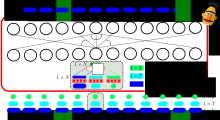
\includegraphics[width=0.95\textwidth]{../../img/word-sem/bert-arch.pdf}
		\end{center}
	\end{frame}

	\begin{frame}
		\frametitle{ML for NLP: \insertsection}
		\framesubtitle{\insertsubsection: Pretrained models (GPT: Dec) \cite{radford2018improving}}
		\begin{figure}[htbp]
			\hgraphpage[\textwidth]{gpt-arch_.pdf}
			\caption{GPT's architecture and different tasks \cite{radford2018improving}}
		\end{figure}
	\end{frame}

	\begin{frame}
		\frametitle{ML for NLP: \insertsection}
		\framesubtitle{\insertsubsection: Pretrained models (T5: Enc-Dec) \cite{T5}}
		\begin{figure}[htbp]
			\hgraphpage[\textwidth]{t5-arch_.pdf}
			\caption{T5's (Text-to-Text Transfer Transformer) training \cite{T5}}
		\end{figure}
	\end{frame}

	\begin{frame}
		\frametitle{ML for NLP: \insertsection}
		\framesubtitle{\insertsubsection: Pretrained models (BART: Enc-Dec) \cite{bart}}
		\begin{figure}[htbp]
			\centering
			\hgraphpage[0.58\textwidth]{bart-arch1_.pdf}
			\hgraphpage[0.4\textwidth]{bart-arch2_.pdf}
			\caption{BART's training \cite{bart}}
		\end{figure}
	\end{frame}


	\begin{frame}
		\frametitle{ML for NLP: \insertsection}
		\framesubtitle{\insertsubsection: Some humor}
		\begin{center}
			\vgraphpage{humor/humor-transformer.png}
		\end{center}
	\end{frame}

	
	\insertbibliography{NLP02}{*}
	
\end{document}

